 \documentclass [12pt]{article} 

\usepackage {amsmath}
\usepackage {amsthm}
\usepackage {amssymb}
\usepackage {graphicx} 
\usepackage {float}
\usepackage {multirow}
\usepackage {xcolor}
\usepackage {algorithmic}
\usepackage [ruled,vlined,commentsnumbered,titlenotnumbered]{algorithm2e} \usepackage {array} 
\usepackage {booktabs} 
\usepackage {url} 
\usepackage {parskip} 
\usepackage [margin=1in]{geometry} 
\usepackage [T1]{fontenc} 
\usepackage {cmbright} 
\usepackage [many]{tcolorbox} 
\usepackage [colorlinks = true,
            linkcolor = blue,
            urlcolor  = blue,
            citecolor = blue,
            anchorcolor = blue]{hyperref} 
\usepackage {enumitem} 
\usepackage {xparse} 
\usepackage {verbatim}
\usepackage{listings}
\usepackage{xcolor}
\lstset { %
    language=C++,
    backgroundcolor=\color{black!5}, % set backgroundcolor
    basicstyle=\footnotesize,% basic font setting
}
\newtheorem{theorem}{Theorem}
\newtheorem{remark}{Remark}



\DeclareTColorBox {Solution}{}{breakable, title={Solution}} \DeclareTColorBox {Solution*}{}{breakable, title={Solution (provided)}} \DeclareTColorBox {Instruction}{}{boxrule=0pt, boxsep=0pt, left=0.5em, right=0.5em, top=0.5em, bottom=0.5em, arc=0pt, toprule=1pt, bottomrule=1pt} \DeclareDocumentCommand {\Expecting }{+m}{\textbf {[We are expecting:} #1\textbf {]}} \DeclareDocumentCommand {\Points }{m}{\textbf {(#1 pt.)}} 

\begin {document} 

\vspace {1em} 
\begin {Instruction} 
Adapted From Virginia Williams' lecture notes.
\end {Instruction}  

{\LARGE \textbf {COMP 285 (NC A\&T, Spr `22)}\hfill \textbf {Lecture 12} } 

\begin{centering}
\section*{Data Structures: Heaps and Red-Black Trees}
\end{centering}

\section{Introduction}
From last lecture, we learned about Sorted Arrays and Linked lists as data structures to store data. In this lecture, we'll sketch out another data structure. It should be mainly review from COMP 280, though we will go into more rigorous detail to proof our claims.

We will sketch out the Binary Search Tree. Before talking about binary search trees, we sketch another data structure called Heap. Heaps are worse than both unsorted linked lists and sorted arrays in just about any parameter, except that they can allow for efficient ($O(\log n)$ time) insertions - still worse than linked lists. But there is one operation that Heaps do exceptionally well (again, $\Theta(\log n)$): \texttt{extract-min}, which outputs the minimum element, and then deletes it from the heap. Heaps (in their simple form that we consider here) still don't beat the asymptotic runtime of binary search trees for any operation, but they have two other advantages: they are much simpler, and if you only want to run insert and \texttt{extract-min} they are also much faster in practice.

\section{Heaps} \textbf{Definition} (Complete binary tree). A complete binary tree is a rooted binary tree where each level is full except maybe the last level, and all nodes on the last level are as far left as they can be.

\textbf{Definition} (Binary min-heap). 

A \textit{Binary min-heap} is a data structure that stores elements that have keys from a totally ordered universe (say, the integers). A binary min-heap supports the following operations: 

\begin{itemize}
  \item \texttt{insert}(i): Inserts an element with key $i$ into the data structure
  \item \texttt{extract-min}: Returns the element with the minimum key and deletes it from the data structure. 
\end{itemize}

A binary heap stores elements in a complete binary tree with a root $r$. Each node $x$ has key($x$) (the key of the element stored in $x$), p($x$) (the parent of $x$, where p($r$) = NIL), left($x$) (the left child of $x$), and right($x$) (the right child of $x$). The children of $x$ are either other nodes or NIL.

A binary heap should satisfy two key properties: The first key property is that for every node $x$, the keys of all nodes under $x$ are greater than key($x$). The second key property of a heap is that its tree is complete (see 1). 

As explained above, binary min-heaps (which we call heaps for short) support two operations3 : \texttt{insert}(i) and \texttt{extract-min}. These are particularly useful if you want to have a priority queue where elements (e.g. jobs) arrive in an arbitrary order, but always leave in order of their key/priority (e.g. when the highest priority job is executed first).

\subsection{Basic Operations on Heaps}
In the heap data structure we always maintain a pointer to the last node in the heap (the right most node in the last level), as well as a pointer to the next node to be created (typically the one to the right of the last node; except when the last level is full, in which case this is the left-most node in the next level). Maintaining those is easy when we think of the
representation of a heap as an array. But to make things simpler, we will abstract these details and simply assume access to these pointers. (See CLRS for details.)

\subsubsection{\texttt{insert}(i)} 
To insert an element, we create a new node with key $i$ at the bottom of the heap. Then recursively “propagate it up the heap” until the heap property is restored: That is compare i to the key of the new element's parent; if $i$ is smaller than the key of its parent, replace the keys, and continue to compare with the parent's parent, etc. Once the algorithm reaches a parent whose key is smaller, the insertion is complete.

\begin{algorithm}
\caption{Heap \texttt{insert}(i)}\label{alg:heap_insert}
\begin{algorithmic}
\STATE $x \gets $ first node without two children
\STATE $y \gets$ new node with key$(y) \gets i$, left$(y) \gets $ NIL, right$(y) \gets $ NIL, $p(y)\gets x$ 
\IF {$left(x) == NIL$}
  \STATE left$(x) \gets y$
\ELSE 
  \STATE right$(x) \gets y$
\ENDIF
\WHILE {$p(y) \neq \text{NIL} \& \text{key}(p(y)) > \text{key}(y)$}
  \STATE $v \gets \text{key}(y)$ 
  \STATE $\text{key}(y) \gets \text{key}(p(y)) $
  \STATE $\text{key}(p(y)) \gets v$
  \STATE $y \gets p(y)$
\ENDWHILE
\end{algorithmic}
\end{algorithm}

\subsubsection{\texttt{extract-min}}
To extract-min, we save the key of the root, replace it with the key of the last node, and delete the last node. Then we recursively ``propagate the key copied from the last node down the tree''. That is compare to the children of the root; if the key of the root is larger than the keys of one of the children, swap the smaller key up, and recurse on the corresponding sub-tree. Once the algorithm reaches children whose keys are larger, the heap property is restored. Then we can return the value we saved at the beginning.

\begin{algorithm}
\caption{Heap \texttt{extract-min}(i)}
\label{alg:heap_extract}
\begin{algorithmic}
\STATE $x \gets $ last node
\STATE $r \gets$ root, $m \gets$ key($r$)
\STATE key($r) \gets $ key($x$)
\IF {right($p(x)$) == NIL}
  \STATE left($p(x)) \gets$ NIL
\ELSE
  \STATE right($p(x)) \gets$ NIL
\ENDIF
delete node($x$)
\WHILE {True}
  \IF {left($r$) == NIL}
    \RETURN m
  \ELSIF{key(left($r$)) $<$ key($r$) \& right($r$) == NIL}
    \STATE $v \gets \text{key}(r)$
    \STATE $\text{key}(r) \gets \text{key}(\text{left}(r))$
    \STATE $\text{key}(\text{left}(r)) \gets v$
    \STATE $r \gets \text{left}(r)$
  \ELSIF{key(left($r$)) $<$ key($r$), key(righ($r$))}
    \STATE $v \gets \text{key}(r)$
    \STATE $\text{key}(r) \gets \text{key}(\text{left}(r))$
    \STATE $\text{key}(\text{left}(r)) \gets v$
    \STATE $r \gets \text{left}(r)$
  \ELSIF{key(right($r$)) $<$ key($r$), key(left($r$))}
    \STATE $v \gets \text{key}(r)$
    \STATE $\text{key}(r) \gets \text{key}(\text{right}(r))$
    \STATE $\text{key}(\text{right}(r)) \gets v$
    \STATE $r \gets \text{right}(r)$
  \ELSE
    \RETURN m
  \ENDIF
\ENDWHILE
\RETURN m

\end{algorithmic}
\end{algorithm}

\section{Binary Search Trees} 
\textbf{Definition} (Binary search tree).

A binary search tree (BST) is a data structure that stores elements that have keys from a totally ordered universe (say, the integers). In this lecture, we will assume that each element has a unique key. A BST supports the following operations: 

\begin{itemize}
  \item search(i): Returns an element in the data structure associated with key i
  \item insert(i): Inserts an element with key i into the data structure
  \item delete(i): Deletes an element with key i from the data structure, if such an element exists
\end{itemize}

A BST stores the elements in a binary tree with a root $r$. Each node $x$ has key($x$) (the key of the element stored in $x$), $p(x)$ (the parent of $x$, where $p(r ) = NIL$), $left(x$) (the left child of $x$), and right($x$) (the right child of $x$). The children of $x$ are either other nodes or NIL.

The key BST property is that for every node $x$, the keys of all nodes under left($x$) are less than key($x$) and the keys of all nodes under right($x$) are greater than key($x$).

\textit{Example 4}. In the following example, the root node $r$ stores $3$ in it (key($r) = 3$), its left child left($x$) stores 1, its right child right($x$) stores 7, and all leaf nodes (storing 1, 4, and 8, respectively) have NIL as their two children.

\begin{center}
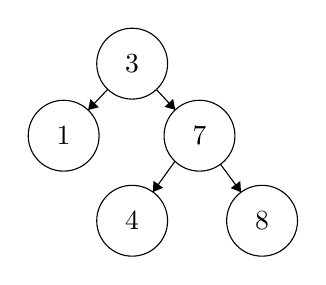
\begin{tikzpicture}[scale=0.15]
\tikzstyle{every node}+=[inner sep=0pt]
\draw [black] (25.7,-16.1) circle (3);
\draw (25.7,-16.1) node {$3$};
\draw [black] (25.7,-29.4) circle (3);
\draw (25.7,-29.4) node {$4$};
\draw [black] (31.4,-22.2) circle (3);
\draw (31.4,-22.2) node {$7$};
\draw [black] (19.9,-22.2) circle (3);
\draw (19.9,-22.2) node {$1$};
\draw [black] (36.7,-29.4) circle (3);
\draw (36.7,-29.4) node {$8$};
\draw [black] (23.63,-18.27) -- (21.97,-20.03);
\fill [black] (21.97,-20.03) -- (22.88,-19.79) -- (22.16,-19.1);
\draw [black] (27.75,-18.29) -- (29.35,-20.01);
\fill [black] (29.35,-20.01) -- (29.17,-19.08) -- (28.44,-19.76);
\draw [black] (29.3,-24.4) -- (27.45,-26.97);
\fill [black] (27.45,-26.97) -- (28.33,-26.61) -- (27.51,-26.02);
\draw [black] (33.18,-24.62) -- (34.92,-26.98);
\fill [black] (34.92,-26.98) -- (34.85,-26.04) -- (34.04,-26.64);
\end{tikzpicture}
\end{center}

Example 5. The following binary tree is not a BST since 2 > 3 and 2 is a child of 7, which is the right child of 3:

\begin{center}
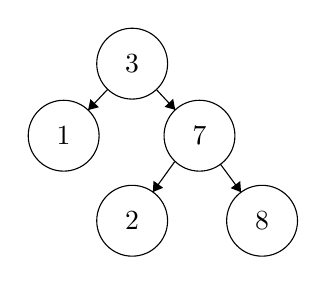
\begin{tikzpicture}[scale=0.15]
\tikzstyle{every node}+=[inner sep=0pt]
\draw [black] (25.7,-16.1) circle (3);
\draw (25.7,-16.1) node {$3$};
\draw [black] (25.7,-29.4) circle (3);
\draw (25.7,-29.4) node {$2$};
\draw [black] (31.4,-22.2) circle (3);
\draw (31.4,-22.2) node {$7$};
\draw [black] (19.9,-22.2) circle (3);
\draw (19.9,-22.2) node {$1$};
\draw [black] (36.7,-29.4) circle (3);
\draw (36.7,-29.4) node {$8$};
\draw [black] (23.63,-18.27) -- (21.97,-20.03);
\fill [black] (21.97,-20.03) -- (22.88,-19.79) -- (22.16,-19.1);
\draw [black] (27.75,-18.29) -- (29.35,-20.01);
\fill [black] (29.35,-20.01) -- (29.17,-19.08) -- (28.44,-19.76);
\draw [black] (29.3,-24.4) -- (27.45,-26.97);
\fill [black] (27.45,-26.97) -- (28.33,-26.61) -- (27.51,-26.02);
\draw [black] (33.18,-24.62) -- (34.92,-26.98);
\fill [black] (34.92,-26.98) -- (34.85,-26.04) -- (34.04,-26.64);
\end{tikzpicture}
\end{center}


\textbf{Some properties.} \textit{Relationship to Quicksort: We can think of each node $x$ as a pivot for quicksort for the keys in its subtree. The left subtree contains $A_<$ for key$(x)$ and the right subtree contains $A_>$ for key($x$).}

\textit{Sorting the keys}: We can do an \textit{inorder} traversal of the tree to recover the nodes in sorted order from left to right (the smallest element is in the leftmost node and the largest element is in the rightmost node). The Inorder procedure takes a node $x$ and returns the keys in the subtree under $x$ in sorted order. We can recursively define Inorder($x$) as: (1) If left$(x) \neq$  NIL, then run Inorder(left$(x)$), then: (2) Output key$(x)$ and then: (3) If right$(x) \neq$ NIL, run Inorder(right$(x)$). With this approach, for every $x$, all keys in its left subtree will be output
before $x$, then $x$ will be output and then every element in its right subtree.

\textit{Subtree property}: If we have a subtree where $x$ has $y$ as a left child, $y$ has $z$ as a right child, and $z$ is the root for the subtree $T_z$ , then our BST property implies that all keys in $T_z$ are $> y $ and $< x$. Similarly, if we have a subtree where $x$ has $y$ as a right child, $y$ has $z$ as a left child, and $z$ is the root of the subtree $T_z$ , then our BST property implies that all keys in $T_z$ are between $x$ and $y$.

\subsection{Basic Operations of BSTs} 
The three core operations on a BST are search, insert, and delete. For this lecture, we will assume that the BST stores distinct numbers, i.e. we will identify the objects with their names and we will have each name be represented by a number.

\subsubsection{search} 
To search for an element, we start at the root and compare the key of the node we are looking at to the element we are searching for. If the node's key matches, then we are done. If not, we recursively search in the left or right subtree of our node depending on whether this node was too large or too small, respectively. If we ever reach NIL, we know the element does not exist in our BST. In the following algorithm in this case, we simply return the node that would be the parent of this node if we inserted it into our tree.


\begin{algorithm}
\caption{\texttt{search}(i)}\label{alg:bst_search}
\begin{algorithmic}
\RETURN search(root, i)
\end{algorithmic}
\end{algorithm}

\begin{algorithm}
\caption{\texttt{search}(x, i)}\label{alg:bst_search_substree}
\begin{algorithmic}
\IF {key(x) == i}
  \RETURN $x$
\ELSIF {key(x) < i}
  \IF {right(x) == NIL}
    \RETURN $x$
  \ENDIF
  \RETURN search(right(x), i)
\ELSIF {key(x) > i}
  \IF {left(x) == NIL} 
    \RETURN $x$
  \ENDIF
  \RETURN search(left(x), i)
\ENDIF
\end{algorithmic}
\end{algorithm}

\textit{Example 6}. If we call \texttt{search}(5.5) on the following BST, we will return the node storing 5 (by taking the path $4 \to 6 \to 5$). This also corresponds to the path taken when calling \texttt{search}(4.5) or
\texttt{search}(5).

\begin{center}
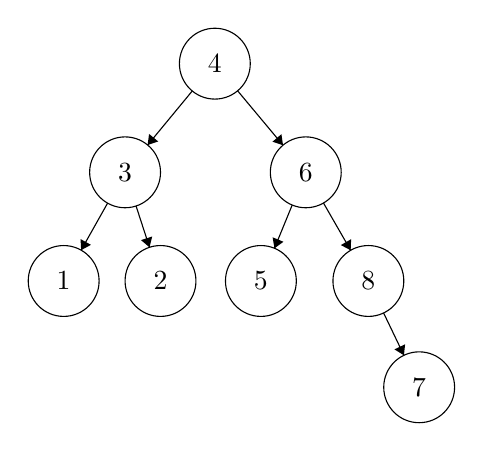
\begin{tikzpicture}[scale=0.15]
\tikzstyle{every node}+=[inner sep=0pt]
\draw [black] (25.2,-16) circle (3);
\draw (25.2,-16) node {$4$};
\draw [black] (17.6,-25.2) circle (3);
\draw (17.6,-25.2) node {$3$};
\draw [black] (12.4,-34.4) circle (3);
\draw (12.4,-34.4) node {$1$};
\draw [black] (20.6,-34.4) circle (3);
\draw (20.6,-34.4) node {$2$};
\draw [black] (32.9,-25.2) circle (3);
\draw (32.9,-25.2) node {$6$};
\draw [black] (38.2,-34.4) circle (3);
\draw (38.2,-34.4) node {$8$};
\draw [black] (29.1,-34.4) circle (3);
\draw (29.1,-34.4) node {$5$};
\draw [black] (42.5,-43.4) circle (3);
\draw (42.5,-43.4) node {$7$};
\draw [black] (23.29,-18.31) -- (19.51,-22.89);
\fill [black] (19.51,-22.89) -- (20.41,-22.59) -- (19.63,-21.95);
\draw [black] (27.13,-18.3) -- (30.97,-22.9);
\fill [black] (30.97,-22.9) -- (30.84,-21.97) -- (30.08,-22.61);
\draw [black] (16.12,-27.81) -- (13.88,-31.79);
\fill [black] (13.88,-31.79) -- (14.71,-31.34) -- (13.83,-30.85);
\draw [black] (18.53,-28.05) -- (19.67,-31.55);
\fill [black] (19.67,-31.55) -- (19.9,-30.63) -- (18.95,-30.94);
\draw [black] (31.75,-27.97) -- (30.25,-31.63);
\fill [black] (30.25,-31.63) -- (31.01,-31.08) -- (30.09,-30.7);
\draw [black] (34.4,-27.8) -- (36.7,-31.8);
\fill [black] (36.7,-31.8) -- (36.74,-30.86) -- (35.87,-31.36);
\draw [black] (39.49,-37.11) -- (41.21,-40.69);
\fill [black] (41.21,-40.69) -- (41.31,-39.76) -- (40.41,-40.19);
\end{tikzpicture}
\end{center}

\textbf{Claim}. \texttt{search}(i) returns a node containing $i$ if $i \in$ BST, otherwise a node $x$ such that either key($x$) is the smallest in BST > $i$ or the largest in BST < $i$, where node $x$ happens to be the parent of the new node if it were to be inserted into BST. This follows directly from
the BST property. Try to formally prove this claim as an exercise.

\begin{center}
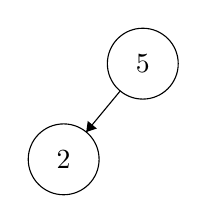
\begin{tikzpicture}[scale=0.15]
\tikzstyle{every node}+=[inner sep=0pt]
\draw [black] (25.2,-16) circle (3);
\draw (25.2,-16) node {$5$};
\draw [black] (18.5,-24.1) circle (3);
\draw (18.5,-24.1) node {$2$};
\draw [black] (23.29,-18.31) -- (20.41,-21.79);
\fill [black] (20.41,-21.79) -- (21.31,-21.49) -- (20.54,-20.85);
\end{tikzpicture}
\end{center}

\textit{Remark 8}. \texttt{search}(i) does not necessarily return the node in BST that is closest in value. Consider the tree above. If we \texttt{search}for an element with a key of 4, the node with key 2 is returned, whereas the element with key 5 is the closest element by value

\subsubsection{insert}
As before, we will assume that all keys are distinct. We will search(i) for a node $x$ to be the parent and create a new node y , placing it as a child of $x$ where it would logically go according to the BST property.

\begin{algorithm}
\caption{\texttt{insert}(i)}\label{alg:bst_inert}
\begin{algorithmic}
\STATE $x \gets $ search(i)
\STATE $y \gets$ new node with key$(y) \gets i$, left$(y) \gets$ NIL, right($y) \gets$ NIL, $p(y) \gets x$
\IF {i < key(x)}
  \STATE left$(x) \gets y$
\ELSE
  \STATE right$(x) \gets y$
\ENDIF
\end{algorithmic}
\end{algorithm}

\textit{Remark 9}. Notice that $x$ needed to have NIL as a child where we want to put $y$ by the properties of our search algorithm

\subsubsection{delete}
Deletion is a bit more complicated. To delete a node $x$ that exists in our tree, we consider several cases:
\begin{enumerate}
  \item If $x$ has no children, we simply remove it by modifying its parent to replace $x$ with NIL.
  \item If $x$ has only one child c, either left or right, then we elevate c to take $x$'s position in the tree by modifying the appropriate pointer of $x$'s parent to replace $x$ with c, and also fixing c's parent pointer to be $x$'s parent.
  \item  If $x$ has two children, a left child $c_1$ and right child $c_2$, then we find $x$'s immediate successor $z$ and have $z$ take $x$'s position in the tree. Notice that $z$ is in the subtree under $x$'s right child $c_2$ and we can find it by running $z \gets \texttt{search}(c_2, key(x))$. Note that since $z$ is $x$'s successor, it doesn't have a left child, but it might have a right child. If $z$ has a right child, then we make $z$'s parent point to that child instead of z (also fixing the child's parent pointer). Then we replace $x$ with z, fixing up all relevant pointers: the rest of $x$'s original right subtree becomes z's new right subtree, and $x$'s left subtree becomes z's new left subtree. (Note that alternatively, we could have used $x$'s immediate predecessor y and followed the same analysis in a mirrored fashion.)

\end{enumerate}
In the following algorithm, if $p$ is the parent of $x$, $child(p)$ refers to $left(p)$ if $x$ was the left child of $p$ and to $right(p)$ otherwise.

\begin{algorithm}
\caption{\texttt{delete}(i)}\label{alg:bst_delete}
\begin{algorithmic}
\STATE $x \gets $ search(i)
\IF {key(x) $\neq i$}
  \RETURN
\ENDIF
\IF {NIL = left(x) and NIL = right(x)} 
  \STATE child(p(x)) $\gets$ NIL
  \STATE delete-node(x)
\ENDIF
\IF {NIL = left(x)}
  \STATE $y \gets $ right(x)
  \STATE $p(y) \gets p(x)$
  \STATE $child(p(y)) \gets y$
  \STATE delete-node(x)
\ELSIF {NIL = right(x)}
  \STATE $y \gets $ right(x)
  \STATE $p(y) \gets p(x)$
  \STATE $child(p(y)) \gets y$
  \STATE delete-node(x)
\ELSE
  \STATE $z \gets $ search(right(x), key(x))
  \STATE $z' \gets$ right(z)
  \STATE left($p(z)) \gets z'$
  \STATE $p(z') \gets p(z)$
  \STATE replace $x$ with $z$
  \STATE delete-node(x)
\ENDIF
\end{algorithmic}
\end{algorithm}


\subsubsection{Runtimes} 
The worst-case runtime for search is $O(\text{height of tree})$. As both insert and delete call search a constant number of times (once or twice) and otherwise perform $O(1)$ work on top of that, their runtimes are also $O(\text{height of tree})$. In the best case, the height of the tree is $O(\log n)$, e.g., when the tree is completely balanced. However, in the worst case it can be $O(n)$ (a long rightward path, for example). This could happen because insert can increase the height of the tree by 1 every time it is called. Currently our operations do not guarantee logarithmic runtimes. To get $O(\log n)$ height we would need to rebalance our tree. There are many examples of self-balancing BSTs, including AVL trees, red-black trees, splay trees (somewhat different but super cool!), etc. Today, we will talk about red-black trees.

\section{Red-Black Trees}
One of the most popular balanced BST is the red-black tree developed by Guibas and Sedgewick in 1978. In a red-black tree, all leaves are assumed to have NILs as children.

\textbf{Definition}. A red-black tree is a BST with the following additional properties:

\begin{enumerate}
  \item Every node is red or black
  \item The root is black
  \item NILs are black
  \item The children of a red node are black
  \item For every node $x$, all $x$ to NIL paths have the same number of black nodes on them
\end{enumerate}

\textit{Example}  (B means a node is black, R means a node is red.) The following tree is not a red-black tree since property 5 is not satisfied:

\begin{center}
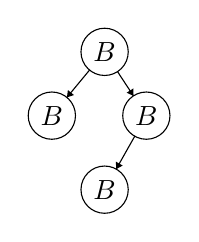
\begin{tikzpicture}[scale=0.1]
\tikzstyle{every node}+=[inner sep=0pt]
\draw [black] (25.2,-16) circle (3);
\draw (25.2,-16) node {$B$};
\draw [black] (18.5,-24.1) circle (3);
\draw (18.5,-24.1) node {$B$};
\draw [black] (30.5,-24.1) circle (3);
\draw (30.5,-24.1) node {$B$};
\draw [black] (25.2,-33.5) circle (3);
\draw (25.2,-33.5) node {$B$};
\draw [black] (23.29,-18.31) -- (20.41,-21.79);
\fill [black] (20.41,-21.79) -- (21.31,-21.49) -- (20.54,-20.85);
\draw [black] (26.84,-18.51) -- (28.86,-21.59);
\fill [black] (28.86,-21.59) -- (28.84,-20.65) -- (28,-21.19);
\draw [black] (29.03,-26.71) -- (26.67,-30.89);
\fill [black] (26.67,-30.89) -- (27.5,-30.44) -- (26.63,-29.94);
\end{tikzpicture}
\end{center}


\textit{Example}. (B means a node is black, R means a node is red.) The following tree is a
red-black tree since all the properties are satisfied:


\begin{center}
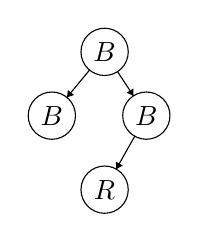
\begin{tikzpicture}[scale=0.1]
\tikzstyle{every node}+=[inner sep=0pt]
\draw [black] (25.2,-16) circle (3);
\draw (25.2,-16) node {$B$};
\draw [black] (18.5,-24.1) circle (3);
\draw (18.5,-24.1) node {$B$};
\draw [black] (30.5,-24.1) circle (3);
\draw (30.5,-24.1) node {$B$};
\draw [black] (25.2,-33.5) circle (3);
\draw (25.2,-33.5) node {$R$};
\draw [black] (23.29,-18.31) -- (20.41,-21.79);
\fill [black] (20.41,-21.79) -- (21.31,-21.49) -- (20.54,-20.85);
\draw [black] (26.84,-18.51) -- (28.86,-21.59);
\fill [black] (28.86,-21.59) -- (28.84,-20.65) -- (28,-21.19);
\draw [black] (29.03,-26.71) -- (26.67,-30.89);
\fill [black] (26.67,-30.89) -- (27.5,-30.44) -- (26.63,-29.94);
\end{tikzpicture}
\end{center}

\textit{Example}. (B means a node is black, R means a node is red.) The following tree is not a
red-black tree since property 4 is not satisfied:

\begin{center}
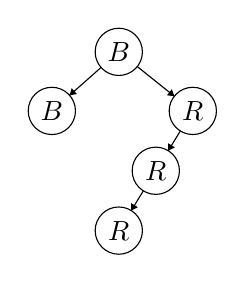
\begin{tikzpicture}[scale=0.1]
\tikzstyle{every node}+=[inner sep=0pt]
\draw [black] (28.3,-15.5) circle (3);
\draw (28.3,-15.5) node {$B$};
\draw [black] (19.8,-23) circle (3);
\draw (19.8,-23) node {$B$};
\draw [black] (37.7,-23) circle (3);
\draw (37.7,-23) node {$R$};
\draw [black] (33,-30.6) circle (3);
\draw (33,-30.6) node {$R$};
\draw [black] (28.3,-38.2) circle (3);
\draw (28.3,-38.2) node {$R$};
\draw [black] (26.05,-17.48) -- (22.05,-21.02);
\fill [black] (22.05,-21.02) -- (22.98,-20.86) -- (22.32,-20.11);
\draw [black] (30.65,-17.37) -- (35.35,-21.13);
\fill [black] (35.35,-21.13) -- (35.04,-20.24) -- (34.42,-21.02);
\draw [black] (36.12,-25.55) -- (34.58,-28.05);
\fill [black] (34.58,-28.05) -- (35.42,-27.63) -- (34.57,-27.11);
\draw [black] (31.42,-33.15) -- (29.88,-35.65);
\fill [black] (29.88,-35.65) -- (30.72,-35.23) -- (29.87,-34.71);
\end{tikzpicture}
\end{center}

\textit{Example}. (B means a node is black, R means a node is red.) The following tree is a
red-black tree:

\begin{center}
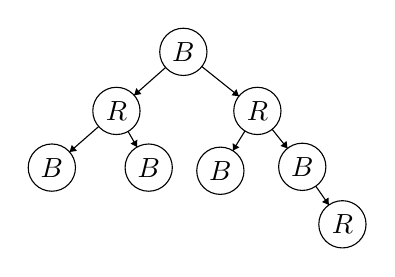
\begin{tikzpicture}[scale=0.1]
\tikzstyle{every node}+=[inner sep=0pt]
\draw [black] (28.3,-15.5) circle (3);
\draw (28.3,-15.5) node {$B$};
\draw [black] (19.8,-23) circle (3);
\draw (19.8,-23) node {$R$};
\draw [black] (37.7,-23) circle (3);
\draw (37.7,-23) node {$R$};
\draw [black] (33,-30.6) circle (3);
\draw (33,-30.6) node {$B$};
\draw [black] (11.6,-30.2) circle (3);
\draw (11.6,-30.2) node {$B$};
\draw [black] (23.9,-30.2) circle (3);
\draw (23.9,-30.2) node {$B$};
\draw [black] (43.4,-30.1) circle (3);
\draw (43.4,-30.1) node {$B$};
\draw [black] (48.5,-37.4) circle (3);
\draw (48.5,-37.4) node {$R$};
\draw [black] (26.05,-17.48) -- (22.05,-21.02);
\fill [black] (22.05,-21.02) -- (22.98,-20.86) -- (22.32,-20.11);
\draw [black] (30.65,-17.37) -- (35.35,-21.13);
\fill [black] (35.35,-21.13) -- (35.04,-20.24) -- (34.42,-21.02);
\draw [black] (36.12,-25.55) -- (34.58,-28.05);
\fill [black] (34.58,-28.05) -- (35.42,-27.63) -- (34.57,-27.11);
\draw [black] (17.55,-24.98) -- (13.85,-28.22);
\fill [black] (13.85,-28.22) -- (14.79,-28.07) -- (14.13,-27.32);
\draw [black] (21.28,-25.61) -- (22.42,-27.59);
\fill [black] (22.42,-27.59) -- (22.45,-26.65) -- (21.59,-27.15);
\draw [black] (39.58,-25.34) -- (41.52,-27.76);
\fill [black] (41.52,-27.76) -- (41.41,-26.82) -- (40.63,-27.45);
\draw [black] (45.12,-32.56) -- (46.78,-34.94);
\fill [black] (46.78,-34.94) -- (46.73,-34) -- (45.91,-34.57);
\end{tikzpicture}
\end{center}

\textbf{Claim} \textit{Any valid red-black tree on $n$ nodes (non-NIL) has height $\leq 2 \log_2(n + 1) = O(\log n)$.}

\textit{Proof} For some node $x$, let $b(x)$ be the ``black height'' of $x$, which is the number of black nodes on a $x \to$ NIL path excluding $x$. We first show that the number of non-NIL descendants of $x$ is at least $2^
{b(x)} - 1$ (including $x$) via induction on the height of $x$.

Base case: NIL node has $b(x) = 0$ and $2^{0}- 1 = 0$ non-NIL descendants. \checkmark

For our inductive step, let $d(x)$ be the number of non-NIL descendants of $x$. Then
\begin{align*}
  d(x) &= 1 + d(\text{left}(x)) + d(\text{right}(x)) \\
  &\geq 1 + (2^{b(x) - 1} - 1) + (2^{b(x) - 1} - 1) \tag{by induction} \\
  &= 2^{b(x)} - 1 \checkmark
\end{align*}

Notice that $b(x) \geq \frac{h(x)}{2}$ (where $h(x)$ is the height of $x$) since on any root to NIL path there are no two consecutive red nodes, so the number of black nodes is at least the number of red nodes, and hence the black height is at least half of the height. We apply this and the above inequality to the root $r$ (letting $h = h(r )$) to obtain $n \geq 2^{b(r)} - 1 \geq 2^{\frac{h}{2}} - 1$, and hence $h \leq 2 log(n + 1)$. Here is some intuition on why the tree is roughly balanced.
 
\textit{Intuition}: By Property (5) of a red-black tree, all $r \to$ NIL paths have $b(r)$ black nodes (excluding the root). Therefore, all these paths have length $\geq b(r)$. However, they also have length $\leq 2 \cdot b(r)$: by Property (4), the number of red nodes is limited to half of the path, since every red node must be followed by a black node, and hence the number of black nodes is at least half of the length of the path. Hence, the lengths of all paths from $r$ to a NIL are within a factor of $2$ of each other, and the tree must be reasonably balanced. Today we will take a brief look at how the red-black tree properties are maintained. Our coverage here is detailed, but not comprehensive, and meant as a case study. For complete coverage, please refer to Chapter 13 of CLRS.

\subsection{Rotations} Red-black trees, as do other balanced BSTs, use a concept called rotation. A tree rotation restructures the tree shape locally, usually for the purpose of balancing the tree better. A rotation preserves the BST property (as shown in the following two diagrams). Notably, tree rotations can be performed in $O(1)$ time.

\begin{center}
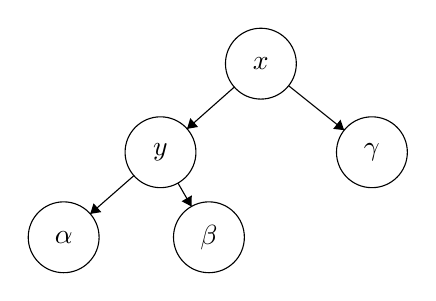
\begin{tikzpicture}[scale=0.15]
\tikzstyle{every node}+=[inner sep=0pt]
\draw [black] (28.3,-15.5) circle (3);
\draw (28.3,-15.5) node {$x$};
\draw [black] (19.8,-23) circle (3);
\draw (19.8,-23) node {$y$};
\draw [black] (37.7,-23) circle (3);
\draw (37.7,-23) node {$\gamma$};
\draw [black] (11.6,-30.2) circle (3);
\draw (11.6,-30.2) node {$\alpha$};
\draw [black] (23.9,-30.2) circle (3);
\draw (23.9,-30.2) node {$\beta$};
\draw [black] (26.05,-17.48) -- (22.05,-21.02);
\fill [black] (22.05,-21.02) -- (22.98,-20.86) -- (22.32,-20.11);
\draw [black] (30.65,-17.37) -- (35.35,-21.13);
\fill [black] (35.35,-21.13) -- (35.04,-20.24) -- (34.42,-21.02);
\draw [black] (17.55,-24.98) -- (13.85,-28.22);
\fill [black] (13.85,-28.22) -- (14.79,-28.07) -- (14.13,-27.32);
\draw [black] (21.28,-25.61) -- (22.42,-27.59);
\fill [black] (22.42,-27.59) -- (22.45,-26.65) -- (21.59,-27.15);
\end{tikzpicture}
\end{center}


\begin{center}
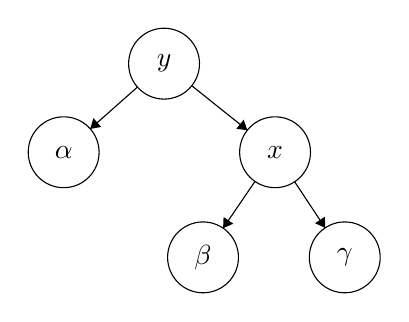
\begin{tikzpicture}[scale=0.15]
\tikzstyle{every node}+=[inner sep=0pt]
\draw [black] (28.3,-15.5) circle (3);
\draw (28.3,-15.5) node {$y$};
\draw [black] (19.8,-23) circle (3);
\draw (19.8,-23) node {$\alpha$};
\draw [black] (37.7,-23) circle (3);
\draw (37.7,-23) node {$x$};
\draw [black] (31.6,-31.9) circle (3);
\draw (31.6,-31.9) node {$\beta$};
\draw [black] (43.6,-31.9) circle (3);
\draw (43.6,-31.9) node {$\gamma$};
\draw [black] (26.05,-17.48) -- (22.05,-21.02);
\fill [black] (22.05,-21.02) -- (22.98,-20.86) -- (22.32,-20.11);
\draw [black] (30.65,-17.37) -- (35.35,-21.13);
\fill [black] (35.35,-21.13) -- (35.04,-20.24) -- (34.42,-21.02);
\draw [black] (36,-25.47) -- (33.3,-29.43);
\fill [black] (33.3,-29.43) -- (34.16,-29.05) -- (33.34,-28.48);
\draw [black] (39.36,-25.5) -- (41.94,-29.4);
\fill [black] (41.94,-29.4) -- (41.92,-28.46) -- (41.08,-29.01);
\end{tikzpicture}
\end{center}

Moving from the first tree to the second is known as a right rotation of $x$. The other direction (from the second tree to the first) is a left rotation of $y$. Notice that we only move the $\beta$ subtree, which is why we preserve the BST property.

\subsection{Insertion in a Red-Black Tree}
Let's see how we can perform Insert(i) on a red-black tree while still maintaining all of its properties. The process for inserting a new node is initially similar to that of insertion into any BST.

\begin{algorithm}
\caption{\texttt{insert\_rb}(i)}\label{alg:insert_rb}
\begin{algorithmic}
\STATE $x \gets $ search(i)
\STATE $y \gets$ new node with key$(y) \gets i$, left$(y) \gets$ NIL, right($y) \gets$ NIL, $p(y) \gets x$
\IF {i < key(x)}
  \STATE left$(x) \gets y$
\ELSE
  \STATE right$(x) \gets y$
\ENDIF
\STATE color(x) $\gets $ red
\STATE recolor if needed
\end{algorithmic}
\end{algorithm}

Note that when $x$ is inserted as a red node: Property (1) is satisfied, as we colored the new node red; Property (2) is satisfied, as we did not touch the root; Property (3) is satisfied, as we can color the new NILs black; and Property (5) is satisfied, as we did not change the number of black nodes in the tree. Thus, the only invariant we have to worry about is Property (4), that red nodes have black children. 

The recoloring step is broken down into multiple cases. We consider each of them:

Case 1: p is black. In this case, Property (4) is also maintained. So, we simply add $x$ as a new red child of p, and the red-black tree properties are maintained.

\begin{center}
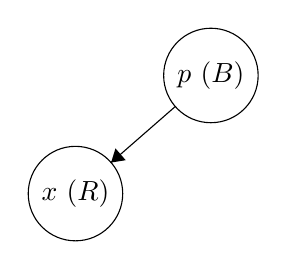
\begin{tikzpicture}[scale=0.2]
\tikzstyle{every node}+=[inner sep=0pt]
\draw [black] (28.3,-15.5) circle (3);
\draw (28.3,-15.5) node {$p\mbox{ }(B)$};
\draw [black] (19.7,-23) circle (3);
\draw (19.7,-23) node {$x\mbox{ }(R)$};
\draw [black] (26.04,-17.47) -- (21.96,-21.03);
\fill [black] (21.96,-21.03) -- (22.89,-20.88) -- (22.24,-20.13);
\end{tikzpicture}
\end{center}

Case 2: p is red, and $x$'s uncle $u$ is red. In this case, we insert a red $x$, change p and $u$ to black, and change p' to red. Because we switched the colors of two nodes on each of these paths (one red $\to$ black and one black $\to$ red), the number of black nodes on each path is unchanged, so Property (5) remains unchanged. If the parent of p' , p'', is black, then Property (4) is maintained. Otherwise, if p'' is red and breaks Property (4) by introducing a ``double-red'' pair of nodes (p' and p''), then we have to recolor recursively starting at p'.

\begin{center}
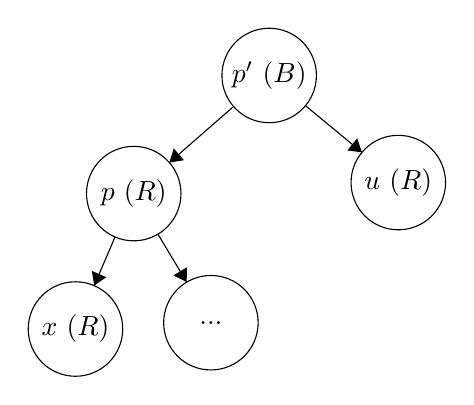
\begin{tikzpicture}[scale=0.2]
\tikzstyle{every node}+=[inner sep=0pt]
\draw [black] (28.3,-15.5) circle (3);
\draw (28.3,-15.5) node {$p'\mbox{ }(B)$};
\draw [black] (19.7,-23) circle (3);
\draw (19.7,-23) node {$p\mbox{ }(R)$};
\draw [black] (16,-31.6) circle (3);
\draw (16,-31.6) node {$x\mbox{ }(R)$};
\draw [black] (24.6,-31.2) circle (3);
\draw (24.6,-31.2) node {$...$};
\draw [black] (36.5,-22.3) circle (3);
\draw (36.5,-22.3) node {$u\mbox{ }(R)$};
\draw [black] (26.04,-17.47) -- (21.96,-21.03);
\fill [black] (21.96,-21.03) -- (22.89,-20.88) -- (22.24,-20.13);
\draw [black] (18.51,-25.76) -- (17.19,-28.84);
\fill [black] (17.19,-28.84) -- (17.96,-28.31) -- (17.04,-27.91);
\draw [black] (21.24,-25.58) -- (23.06,-28.62);
\fill [black] (23.06,-28.62) -- (23.08,-27.68) -- (22.22,-28.19);
\draw [black] (30.61,-17.42) -- (34.19,-20.38);
\fill [black] (34.19,-20.38) -- (33.89,-19.49) -- (33.26,-20.26);
\end{tikzpicture}
\end{center} becomes \begin{center}
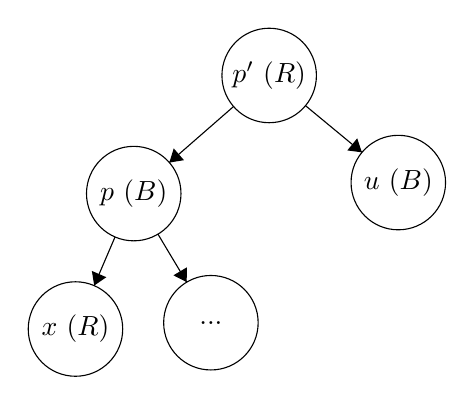
\begin{tikzpicture}[scale=0.2]
\tikzstyle{every node}+=[inner sep=0pt]
\draw [black] (28.3,-15.5) circle (3);
\draw (28.3,-15.5) node {$p'\mbox{ }(R)$};
\draw [black] (19.7,-23) circle (3);
\draw (19.7,-23) node {$p\mbox{ }(B)$};
\draw [black] (16,-31.6) circle (3);
\draw (16,-31.6) node {$x\mbox{ }(R)$};
\draw [black] (24.6,-31.2) circle (3);
\draw (24.6,-31.2) node {$...$};
\draw [black] (36.5,-22.3) circle (3);
\draw (36.5,-22.3) node {$u\mbox{ }(B)$};
\draw [black] (26.04,-17.47) -- (21.96,-21.03);
\fill [black] (21.96,-21.03) -- (22.89,-20.88) -- (22.24,-20.13);
\draw [black] (18.51,-25.76) -- (17.19,-28.84);
\fill [black] (17.19,-28.84) -- (17.96,-28.31) -- (17.04,-27.91);
\draw [black] (21.24,-25.58) -- (23.06,-28.62);
\fill [black] (23.06,-28.62) -- (23.08,-27.68) -- (22.22,-28.19);
\draw [black] (30.61,-17.42) -- (34.19,-20.38);
\fill [black] (34.19,-20.38) -- (33.89,-19.49) -- (33.26,-20.26);
\end{tikzpicture}
\end{center}

Case 3: p is red, and $u$ is black. There are two possibilities here:

\begin{enumerate}
  \item We are inserting $x$ as a leaf node. Then, $u$ must be NIL for the red-black tree to have been valid before inserting $x$. We insert a red $x$.
  \item We are not inserting $x$; rather, we are recoloring the tree at $x$ from the recursive call in Case 2. We aim to recolor the tree and maintain the number of black nodes on each path from the root to NIL. Note that in this case, $x$ actually has nodes under it.
\end{enumerate}

In both cases, $x$ is red, so we make p black, make p' red, and do a right rotation at p' . We can see that this also maintains the same number of black nodes on each path from the root to NIL, and satisfies Property (4) below p because the original tree was a red-black tree.

\begin{center}
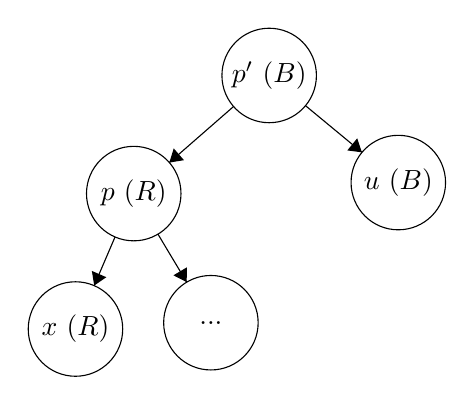
\begin{tikzpicture}[scale=0.2]
\tikzstyle{every node}+=[inner sep=0pt]
\draw [black] (28.3,-15.5) circle (3);
\draw (28.3,-15.5) node {$p'\mbox{ }(B)$};
\draw [black] (19.7,-23) circle (3);
\draw (19.7,-23) node {$p\mbox{ }(R)$};
\draw [black] (16,-31.6) circle (3);
\draw (16,-31.6) node {$x\mbox{ }(R)$};
\draw [black] (24.6,-31.2) circle (3);
\draw (24.6,-31.2) node {$...$};
\draw [black] (36.5,-22.3) circle (3);
\draw (36.5,-22.3) node {$u\mbox{ }(B)$};
\draw [black] (26.04,-17.47) -- (21.96,-21.03);
\fill [black] (21.96,-21.03) -- (22.89,-20.88) -- (22.24,-20.13);
\draw [black] (18.51,-25.76) -- (17.19,-28.84);
\fill [black] (17.19,-28.84) -- (17.96,-28.31) -- (17.04,-27.91);
\draw [black] (21.24,-25.58) -- (23.06,-28.62);
\fill [black] (23.06,-28.62) -- (23.08,-27.68) -- (22.22,-28.19);
\draw [black] (30.61,-17.42) -- (34.19,-20.38);
\fill [black] (34.19,-20.38) -- (33.89,-19.49) -- (33.26,-20.26);
\end{tikzpicture}
\end{center}

becomes

\begin{center}
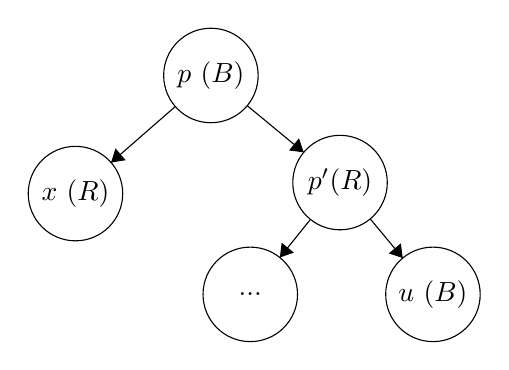
\begin{tikzpicture}[scale=0.2]
\tikzstyle{every node}+=[inner sep=0pt]
\draw [black] (28.3,-15.5) circle (3);
\draw (28.3,-15.5) node {$p\mbox{ }(B)$};
\draw [black] (19.7,-23) circle (3);
\draw (19.7,-23) node {$x\mbox{ }(R)$};
\draw [black] (36.5,-22.3) circle (3);
\draw (36.5,-22.3) node {$p'(R)$};
\draw [black] (30.8,-29.4) circle (3);
\draw (30.8,-29.4) node {$...$};
\draw [black] (42.4,-29.4) circle (3);
\draw (42.4,-29.4) node {$u\mbox{ }(B)$};
\draw [black] (26.04,-17.47) -- (21.96,-21.03);
\fill [black] (21.96,-21.03) -- (22.89,-20.88) -- (22.24,-20.13);
\draw [black] (30.61,-17.42) -- (34.19,-20.38);
\fill [black] (34.19,-20.38) -- (33.89,-19.49) -- (33.26,-20.26);
\draw [black] (34.62,-24.64) -- (32.68,-27.06);
\fill [black] (32.68,-27.06) -- (33.57,-26.75) -- (32.79,-26.12);
\draw [black] (38.42,-24.61) -- (40.48,-27.09);
\fill [black] (40.48,-27.09) -- (40.36,-26.16) -- (39.59,-26.8);
\end{tikzpicture}
\end{center}

If we end up in Case 2 and recursively call recolor, then in the worst case the recursion will bottom out when we hit the root, with a constant number of relabelings and rotations ateach level. So, it will be an $O(h)$ operation overall, where $h$ is the height of the tree.

In the analysis above, we considered the cases where $x$ is a left child of $p$ and $u$ is a rightchild of its parent $p'$. These cases are representative, showing most of the machinery that we’ll need to insert an arbitrary element into an arbitrary red-black tree. (Within Case 2 and Case 3, there are actually a total of four cases each, where p's tree and p`'s children could each be swapped, but the recoloring procedure is similar. You are encouraged to read the text for details.)

To summarize, the following is the algorithm for recoloring, in the case where $x$ is a left childand $u$ is a right child.

\begin{algorithm}
\caption{\texttt{recolor}(x)}\label{alg:recolor_rb}
\begin{algorithmic}
\STATE $p \gets $ parent(x)
\IF {black = color(p))}
  \RETURN
\ENDIF

\STATE $p' \gets \text{parent}(p)$
\STATE $u \gets \text{right}(p')$
\IF {red = color(u) }
  \STATE color(p) $\gets $ black
  \STATE color(u) $\gets $ black
  \STATE color(p') $\gets $ red
  \STATE recolor(p')
\ELSIF {black = color(u)}
  \STATE color(p) $\gets $ black
  \STATE color(p') $\gets $ red
  \STATE \texttt{right\_rotate}(p')
\ENDIF
\end{algorithmic}
\end{algorithm}

Based on our analysis above, we can update our red-black trees in $O(h)$ time upon insertion, where $h$ is the height of the tree. The other operations are similar, and also give the guarantee of worst-case performance of $O(h)$ search, insertion, and deletion. Together with our claim that $h = O(\log n)$, we get:

\textbf{Claim} \textit{Red-Black trees support \texttt{insert}, \texttt{delete}, and \texttt{search} in $O(\log n)$ time}

As we have seen, BSTs are very nice – they allow us to maintain a set and report membership, insert, and delete in $O(\log n)$ time. In addition to these basic underlying operations, we can also support other types of queries efficiently. Because the elements are stored maintaining the binary search tree property, we can search for the next largest element or the elements on a range very efficiently. But what if we don’t care about these properties? What if we only need to support membership queries? Can we improve our performance of $O(\log n)$ time to nearly constant time? This question motivates our discussion of hash tables, which we will cover in the next lecture.












\end{document}

